\chapter{User Manual}
\label{chap:ch5}

\section{Account setup and role assignment}
\label{sec:ch5sec1}

\par When first opening the application the user is taken to a Landing screen (as seen in figure \ref{fig:landing-screen}) where he or she would be presented with the option to Sign Up for a new account or Sign In in an existing account. When pressing the Sign Up button is pressed the user is taken to the Sign Up screen where he or she can send a registration request for a new account, as seen in figure \ref{fig:sign-up-screen}.

\begin{figure}
\centering
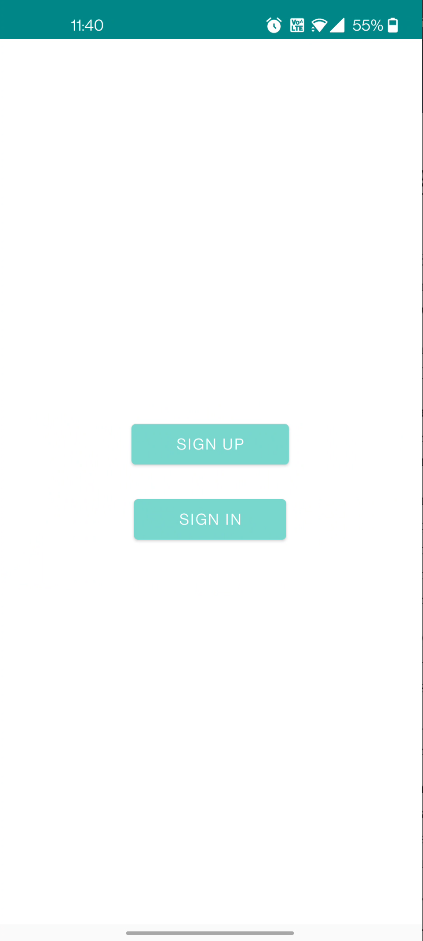
\includegraphics[width=0.4\textwidth]{figures/landing_screen.png}
\caption{The Landing screen}
\label{fig:landing-screen}
\end{figure}

\begin{figure}
\centering
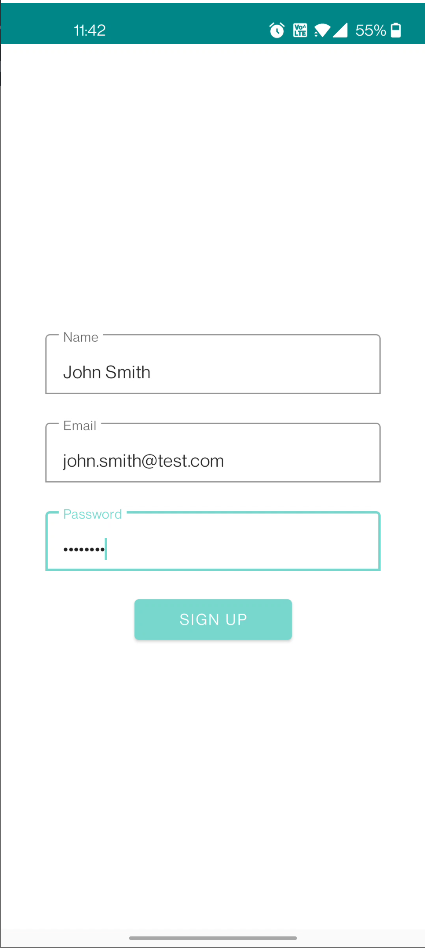
\includegraphics[width=0.4\textwidth]{figures/sign_up_screen.png}
\caption{The Sign Up screen}
\label{fig:sign-up-screen}
\end{figure}

Once this registration is completed, however, the users are still not yet allowed to login into the application as their account needs to be assigned to a specific role. The available roles are the ones seen in the figure \ref{fig:user-role-enum}, except the admin role which is a special role only used to access the dashboard. The admin is the only role that gives an user access to the dashboard where roles can be assigned. The role selection process for our newly created user can be seen in figure \ref{fig:dashboard-assign-role}.

\begin{figure}
\centering
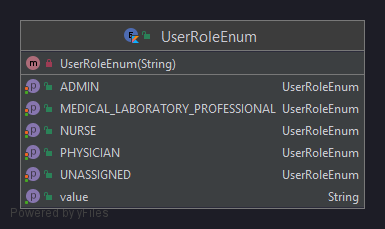
\includegraphics[width=0.75\textwidth]{figures/user-role-enum.png}
\caption{UserRoleEnum Class Diagram}
\label{fig:user-role-enum}
\end{figure}

\begin{figure}
\centering
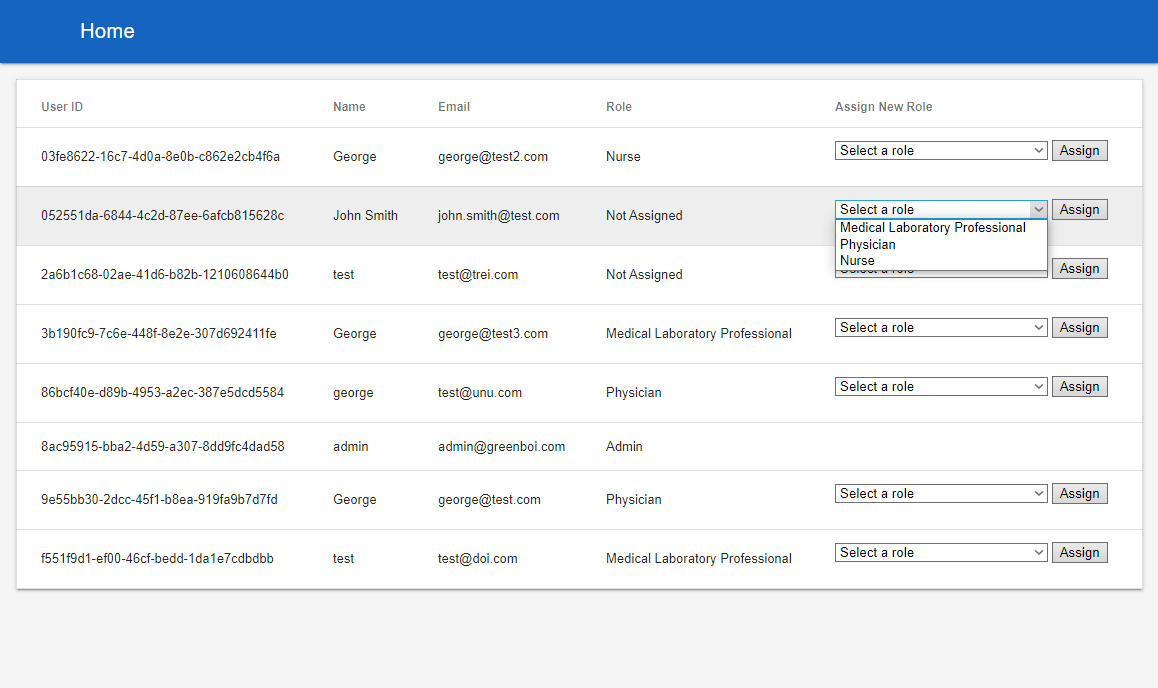
\includegraphics[width=\textwidth]{figures/dashboard_assign_role.png}
\caption{The Admin Dashboard}
\label{fig:dashboard-assign-role}
\end{figure}

\section{Sign In and Home Page}
\label{sec:ch5sec2}

\par In order to Sign In the user needs to go back to the landing screen (figure \ref{fig:landing-screen}) and tap the Sign In button. The user now is being taken to the Sign In screen (figure \ref{fig:sign-in-screen}) where he or she is being asked for the login credentials they have previously created. Once inserted, if they tap the Sign In button a request will be made to the server in order to retrieve an authentication token and the current user's profile.

\begin{figure}
\centering
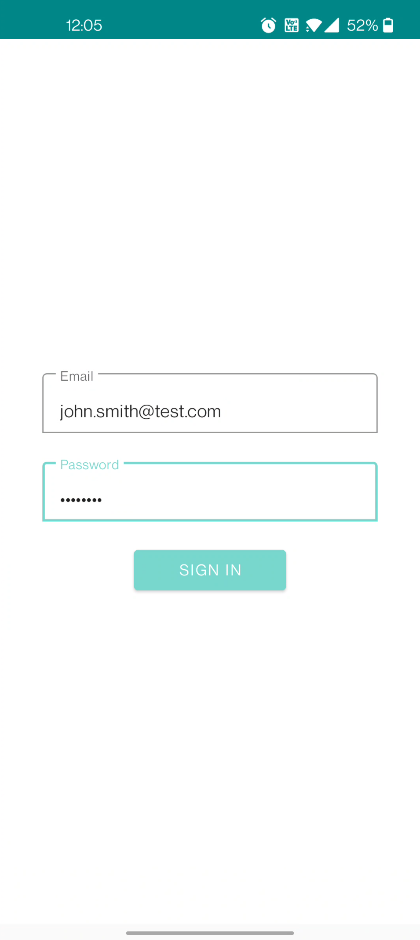
\includegraphics[width=0.4\textwidth]{figures/sign_in_screen.png}
\caption{The Sign In screen}
\label{fig:sign-in-screen}
\end{figure}

After the Sign In process is completed and the required objects are retrieved the user is taken to the home screen (figure \ref{fig:home-screen}). Here the users are presented with some options. The first option is to Sign Out from their account, which, when pressed, will invalidate the user's session and take them back to the landing page. The Second option is to register a patient, which is only available for an account with the Nurse role assigned. The third option is to read a patient's tag.

\begin{figure}
\centering
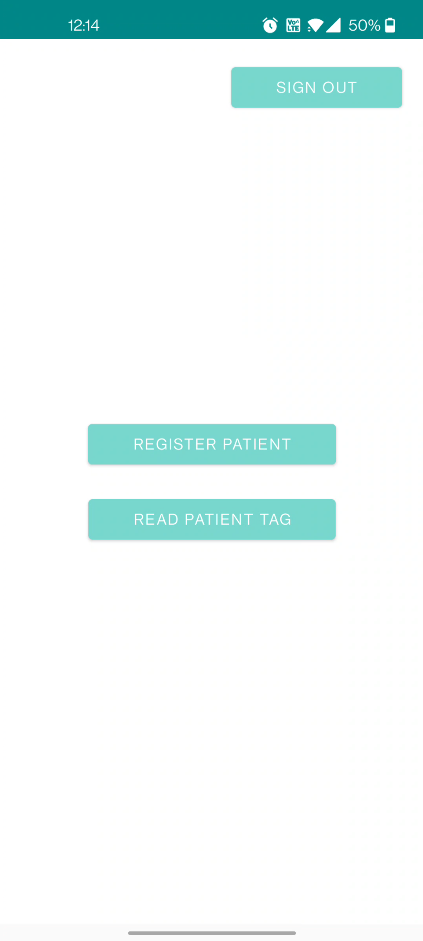
\includegraphics[width=0.4\textwidth]{figures/home_page_screen.png}
\caption{The Home screen}
\label{fig:home-screen}
\end{figure}

\section{Registering a patient}
\label{sec:ch5sec3}

\par When selecting the Register Patient option from the home screen (figure \ref{fig:home-screen}) the user is presented with a form that needs to be completed in order to register a new patient in the database (figure \ref{fig:register-patient-screen}).

\begin{figure}
\centering
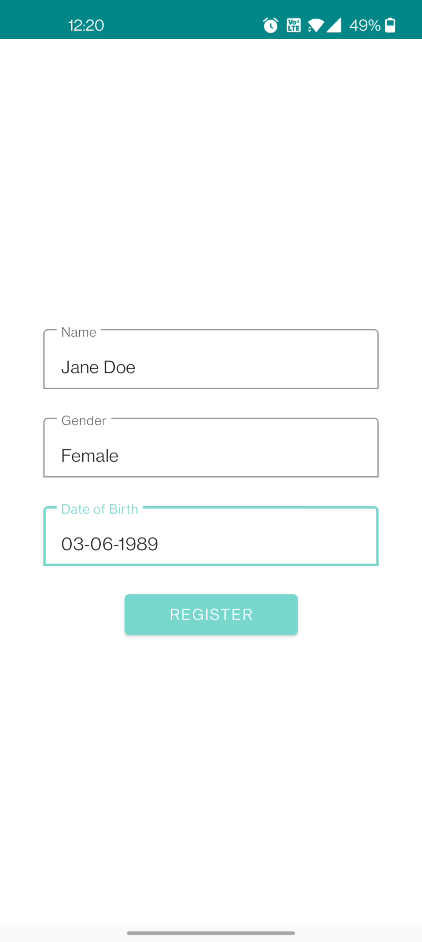
\includegraphics[width=0.4\textwidth]{figures/register_patient_screen.png}
\caption{The Register Patient screen}
\label{fig:register-patient-screen}
\end{figure}

After tapping the register button the nurse is taken to a new screen where she is presented with the possibility of assigning an NFC enabled bracelet to the newly registered patient (figure \ref{fig:write-tag-screen}). As a result of following the instructions that are on the screen the user will be presented with a confirmation dialog, as seen in figure \ref{fig:write-tag-confirmation}. When tapping the Done button the nurse will be automatically taken back to the home page (figure \ref{fig:home-screen}).

\begin{figure}
\centering
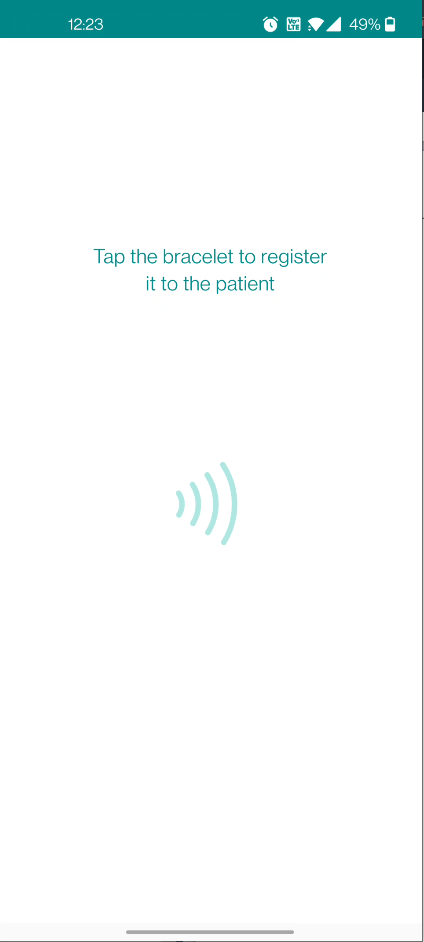
\includegraphics[width=0.4\textwidth]{figures/write_tag_screen.png}
\caption{The Register Tag screen}
\label{fig:write-tag-screen}
\end{figure}

\begin{figure}
\centering
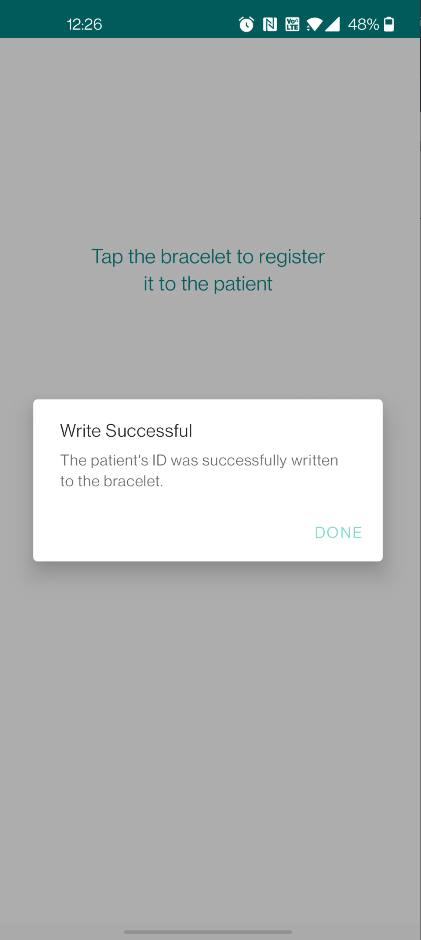
\includegraphics[width=0.4\textwidth]{figures/write_tag_confirmation.png}
\caption{The Register Tag Confirmation}
\label{fig:write-tag-confirmation}
\end{figure}

\section{Retrieving a patient's information}
\label{sec:ch5sec4}

\par In order to retrieve the patient's information the medical personnel is required to tap the Read Patient Tag button found on the home page (figure \ref{fig:home-screen}). Upon doing so, the user is taken to a new screen where he or she is required to close the distance between the device and the bracelet in order to read-off the information from it, as seen in figure \ref{fig:read-tag-screen}. Upon successfully reading the ID stored on the NFC enabled bracelet the patient's information is requested from the server along with a list of generated reports. Once retrieved the user is taken to the View Patient screen (figure \ref{fig:view-patient-screen}).

\begin{figure}
\centering
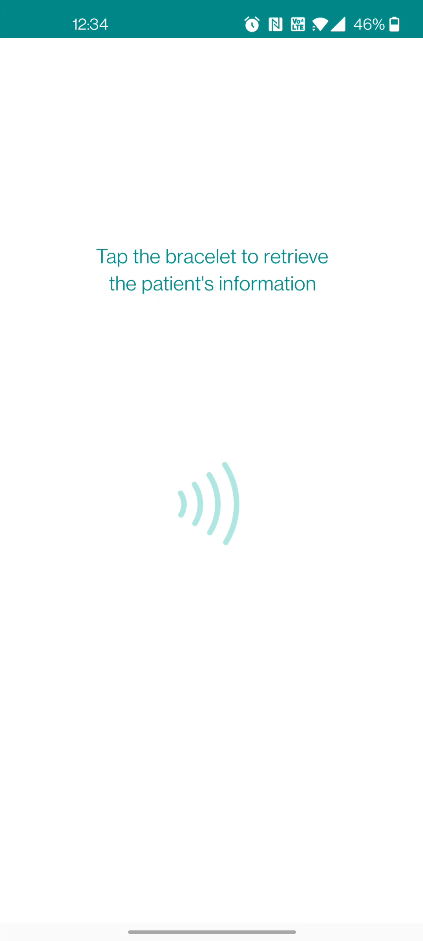
\includegraphics[width=0.4\textwidth]{figures/read_tag_screen.png}
\caption{The Read Patient Tag Screen}
\label{fig:read-tag-screen}
\end{figure}

\begin{figure}
\centering
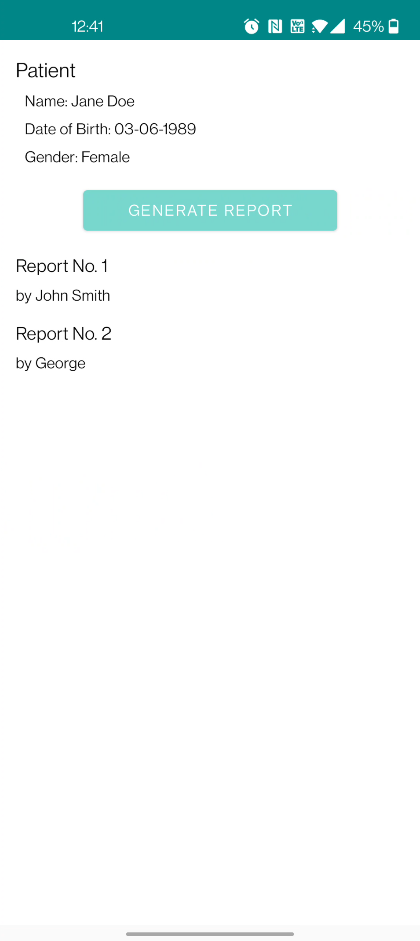
\includegraphics[width=0.4\textwidth]{figures/view_patient_screen.png}
\caption{The View Patient Screen}
\label{fig:view-patient-screen}
\end{figure}

\section{Generating and viewing generated reports}
\label{sec:ch5sec5}

\par When the user is on the View Patient screen, he or she will be able to either view an already generated report from the list seen in figure \ref{fig:view-patient-screen} or generate a new report. Upon selecting a generated report, the details about it are requested from the server and once retrieved, displayed for the medical personnel on a new screen (figure \ref{fig:view-report-screen}).

\begin{figure}
\centering
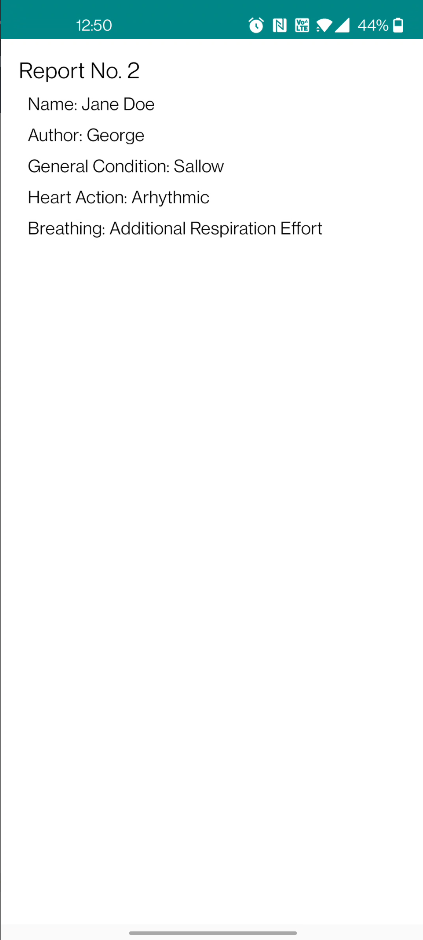
\includegraphics[width=0.4\textwidth]{figures/view_report_screen.png}
\caption{The View Report Screen}
\label{fig:view-report-screen}
\end{figure}

If the medical personnel selects the Generate Report button from the View Patient screen, the user will be presented with a new screen where he or she is able to complete certain information about the state of the patient at the moment when the consultation was done (figure \ref{fig:generate-report-screen}). Upon completing the applicable fields and hitting the Generate button at the bottom of the screen the user will be taken to the view report screen (figure \ref{fig:view-report-screen} which contains the newly generated report.

\begin{figure}
\centering
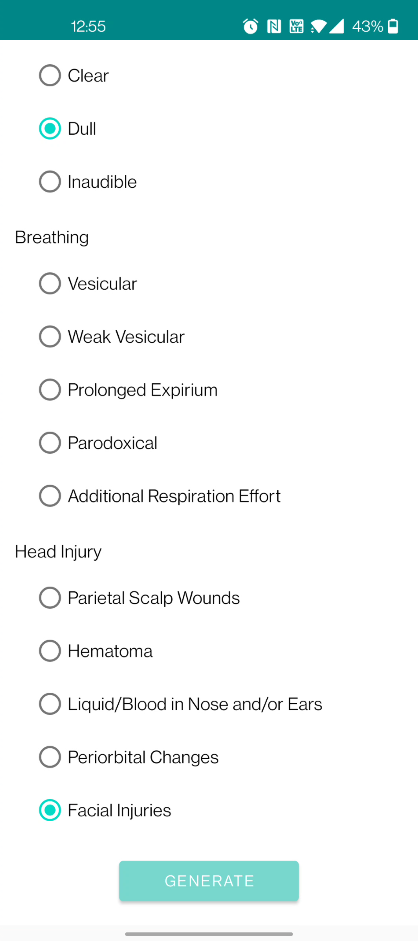
\includegraphics[width=0.4\textwidth]{figures/generate_report_screen.png}
\caption{The Generate Report Screen}
\label{fig:generate-report-screen}
\end{figure}

At the moment of writing this thesis the options for a report consist from some well defined Radio Buttons organized in Radio Groups based on the enum class they are part of. All of the available options can be seen in figure \ref{fig:report-options-diagram}.

\begin{figure}
\centering
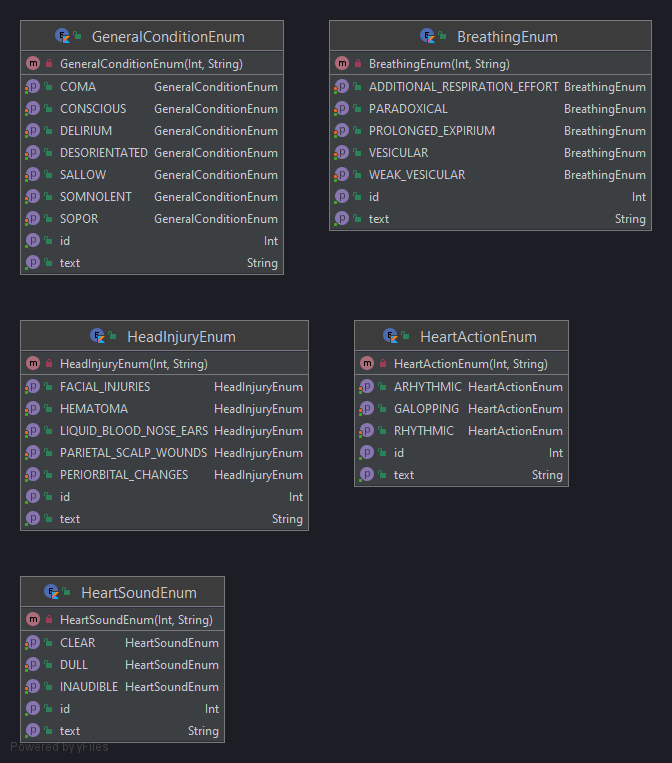
\includegraphics[width=0.75\textwidth]{figures/report_options_class_diagram.png}
\caption{Report Options Class Diagram}
\label{fig:report-options-diagram}
\end{figure}